\documentclass[12pt]{article}
\usepackage{fullpage}
\usepackage{graphicx, rotating, booktabs} 
\usepackage{times} 
\usepackage{fbb} 
\usepackage{natbib} 
\usepackage{indentfirst} 
\usepackage{setspace}
\usepackage{grffile} 
\usepackage{hyperref}
\usepackage{tikz}
\usepackage[export]{adjustbox}
\usepackage[most]{tcolorbox}
\usepackage{verbatimbox}
\usepackage{lscape}
\usepackage{afterpage}
\usepackage{amsmath}
\usepackage[labelfont={bf},textfont=it,labelsep=period]{caption}
 \usepackage{multirow} 
\setcitestyle{aysep{}}
\usepackage{dcolumn}

\hypersetup{
  colorlinks = true,
  urlcolor = blue,
  linkcolor = black,
  citecolor = black,
  pdfauthor = {Joshua Alley},
  pdfkeywords = {},
  pdftitle = {},
  pdfsubject = {},
  pdfpagemode = UseNone,
%  pdffitwindow = true
%  pdfcenterwindow = true
}



\singlespace
\title{\textbf{Alliances, Arms Transfers and Electoral Trade Cycles}}
\author{Joshua Alley \\
Postdoctoral Research Associate \\
University of Virginia\thanks{Thanks to Brian Blankenship, Lauren Peritz, Erik Lin-Greenberg, Zachary Markovitch and participants in the Boston University Political Economy of Security Online Workshop Series for helpful comments.} \\
jkalley@virginia.edu
}

 
\date{\today}

\bibliographystyle{apsr}

\usepackage{sectsty}
\sectionfont{\Large}
\subsectionfont{\noindent\large\textit}
\subsubsectionfont{\normalsize}

\makeatletter
\renewcommand\tiny{\@setfontsize\tiny{9}{10}}
\makeatother


\begin{document}

\maketitle 

\begin{abstract}
What are the international economic and political consequences of political budget cycles? 
Political budget cycles in the United States increase trade and especially drive up exports to allies through arms transfers because defense contracting has an important role in budget cycles. 
%Security cooperation thus shapes the ramifications of political business cycles, as arms transfers to allies contribute to electoral trade cycles in alliance patrons.
When U.S. allies purchase weapons and accept arms transfers, they provide an outlet for outputs from efforts to use defense contracting to stimulate economic growth in key electoral areas.
Alliance proteges thus use positive economic and security statecraft to help patron state leaders manipulate the economy during leadership competitions.  
I test these claims with three analyses of trade, arms transfers and defense contracting in the United States. 
First, I show that U.S. trade follows an electoral cycle, with substantial increases in exports to allies near elections.
I then detail how arms transfers from the United States to allies mirror electoral export cycles. 
Finally, I show that increased defense contract awards around elections lead to arms transfers.
These results suggest that alliance patron leaders can reap electoral benefits from security and economic ties with proteges. 
\end{abstract} 


\newpage 
\doublespace 


\section{Introduction}


% start with a good story of increased trade near elections: compare ally/not 
% Matching for case selection produces: 1996 Denmark and Sweden
U.S. trade with Denmark and Sweden spiked in 1996, as Bill Clinton ran for re-election.
Exports to and imports from both Nordic countries rose, but Denmark received more U.S. exports.
While these countries occupied similar regions, and shared important economic similarities in trade relations with the United States, Denmark received more exports, because U.S. arms transfers to this NATO member also rose in 1996.


% give another example: Turkey and Egypt 1984
Two Middle Eastern states experience similar trade changes in 1984 when Ronald Reagan stood for a second term.
U.S. trade with Turkey and Egypt grew, but exports to Turkey increased more than exports to Egypt. 
As in the Denmark and Sweden case, Turkey had a formal U.S. security guarantee and Egypt did not, so Turkey received greater U.S. arms transfers and higher exports. 


% example- PBC consequences vary w/ security coop
These cases are exemplars of a more general pattern, where presidential elections in the United States expand international economic exchanges, especially exports to allies through arms transfers.
This paper unpacks the role of alliances and arms transfers in electoral trade cycles between the United States and other countries. 
I argue that along with the general increase in trade near presidential elections, U.S. allies receive more exports through arms transfers.


Electoral trade and arms transfer cycles are the result of political business cycles.
Elected leaders often use fiscal and monetary policy \citep{Nordhaus1975, Tufte1978, Rogoff1987, ClarkHallerberg2000} to generate economic growth around elections. 
There is also evidence that leaders use non-budget instruments like social policy \citep{Philips2020}, labor agreements \citep{Ahlquist2010} and trade disputes \citep{Conconietal2017} to win elections. 
Political business cycles in monetary and fiscal policy within large states increase trade. 
Economic expansion pulls in more imports and increases production for export markets. 


% not sure I want the question:
Security cooperation alters the composition of electoral trade cycles. 
Alliance proteges provide a key market for exports from political business cycles in their patron, as they receive more arms purchases and transfers than other states. 
Allies take more arms from their patrons near elections because they control import decisions and U.S. leaders produce additional arms while using defense contracting to create domestic political business cycles \citep{Tufte1978, Mintz1988, Mayer1995, DerouenHeo2000, Becker2021}.
These arms transfer cycles reinforce cooperative relationships between the United States and its alliance proteges.


% Findings
I examine how U.S. allies facilitate electoral export cycles in three ways. 
First, I show that in addition to general electoral trade cycles, allies receive more U.S. exports as presidential elections approach.
I then demonstrate corresponding cycles in arms sales and transfers, where arms transfers to allies rise as elections approach.  
Finally, I show that defense contracting cycles drive U.S. arms exports. 


% focus on the U.S.
The argument and analysis focus on the United States because it has the largest economy, substantial alliance ties, and ample evidence of defense contracting and spending cycles. 
Electoral trade and arms transfer cycles will likely be weaker in other countries with smaller economies and defense industries. 
Still, the pivotal economic and security roles of the United States make understanding the economic and security consequences of U.S. political budget cycles worthwhile.


These claims complement prior findings that foreign states use economic policies to manipulate electoral competition. 
\citet{KimMargalit2021} find that Chinese tariffs reduced Republican vote share in the 2018 midterm elections by targeting industries in competitive districts.
In the same way, \cite{ChyzhUrbatsch2021} find that Chinese soy tariffs hurt Republican congressional candidates in soy-producing areas. 
My argument inverts this logic by examining how security allies accommodate electoral business cycles. 


% economic and seucrity ties 
The argument and findings address three salient issues in international relations theory and practice. 
First, they detail the international consequences of political business cycles. 
Domestic political business cycles in large countries like the United States reshape international economic ties, with knock-on effects in other countries.
International economic expansions and related domestic growth make early elections in parliamentary democracies more likely \citep{Kayser2006} and increase vote shares for parties supporting higher taxes and spending \citep{Kayser2009}, to give two examples.


Second, I speak to debates about how economic and security ties interact \citep{Mastanduno2009, Poast2019}. 
Scholars dispute whether economic linkages drive security ties \citep{BiglaiserDeRouen2007, Fordham2010, Kimball2010}, security concerns encourage economic linkages \citep{Gowa1995, Li2003, LongLeeds2006, GowaMansfield2004}, or both \citep{BiglaiserDeRouen2009, KinneBunte2018}. 
My findings suggest that this relationship changes with electoral cycles.


In asymmetric alliances like those between the United States and its partners, research on economic bargaining usually focuses on patron states' economic leverage, and falls into two camps. 
One argues that alliance patrons have limited economic leverage because they prioritize geopolitical aims \citep{Drezner2013, WolfordKim2017}.
Another perspective claims that alliance leaders have substantial economic influence \citep{Norrlof2010, Brooksetal2013} and threats to reduce security commitment encourage economic concessions \citep[pg. 122]{Oatley2015}.
Rather than analyze coercive economic demands, my argument suggests that arms transfers to proteges around elections help U.S. leaders advance their electoral interests.


% coercion
Finally, this paper provides new insight into economic statecraft. 
Most economic statecraft scholarship studies economic sanctions (e.g. \citep{Marinov2005, Allen2008, Escriba-FolchWright2010}).
But as \citet{Baldwin2020} notes, economic statecraft includes positive inducements and negative sanctions. 
This paper examines positive economic statecraft--- how alliance proteges use political economy decisions to reward patron leaders.
As a result, it assesses issue linkage in alliance management, building on previous work that considers alliance formation \citep{Poast2012} and credibility \citep{Davis2008, Poast2013}. 


% policy 
My findings that allies facilitate political budget cycles through arms exports has important implications for alliance durability. 
Leaders who anticipate benefiting from allied trade cycles will be more likely to demonstrate and uphold alliance commitment. 
Electoral trade cycles are therefore an important component of potential grand bargains between asymmetric alliance patrons and their proteges. 


% need an outline 
The paper proceeds as follows. 
To start, I outline an argument detailing the international economic consequences of political business cycles in large states, the role of defense contracting in those cycles, and the consequences for international trade as well as exports to allies.
I then test the process in three steps. 
First, I show that U.S. exports to allies increase more as elections approach, relative to states without a defense pact. 
I then demonstrate that arms exports from the United States to allies mirror the electoral export cycle.
Third, I establish the political business cycle roots of arms exports with an analysis of defense contracting and arms exports.
The last section discusses the results and offers some concluding thoughts.


\section{Argument}


This argument explains how alliances shape the international consequences of domestic political business cycles. 
First, I detail how political budget cycles expand overall trade.
I then discuss how direct leader control makes defense contracting an attractive policy tool for manipulating economic conditions around elections. 
After that I explain how allies provide an market for outputs from electoral cycles in defense contracting. 
Finally, I detail the net outcome--- general electoral trade cycles with greater exports to allies through arms transfers. 


Electoral considerations impact economic policy \citep{Nordhaus1975}.\footnote{See \citet{Dubois2016} for a review of this extensive literature.} 
Leaders undertake political business cycles by using fiscal and monetary policy to increase economic growth and retain power for themselves or their party \citep{Tufte1978, Rogoff1987}. 
The composition and magnitude of these cycles varies. 
For example, strong central bank interdependence and fixed exchange rates make fiscal cycles more likely \citep{ClarkHallerberg2000}. 
Even some highly independent central banks show some cyclical behavior, however \citep[pg. 247]{Dubois2016}


% Political Business cyles
While business cycles target the domestic economy, they have international economic consequences.
Fiscal and monetary policy shifts impact currency prices and economic activity, which then alters trade and financial ties. 
The larger the cycling economy, the greater the international economic consequences of political business cycles.
Economic interdependence leads to correlated economic growth across countries \citep{ArtisZhang1999, Kayser2006} and increases the global economic influence of large economies. 
\citet{Ito1991} finds that U.S. elections increase economic growth in Japan, while \citet{ThompsonZuk1983} uncover some evidence of similar cycles in advanced industrial economies.
\citet{FoersterSchmitz1997} argue that U.S. electoral cycles shape international stock returns.



% increased domestic consumption- 
There is less empirical evidence of that electoral trade cycles, but the theory is established.
For example, monetary expansion has price and income effects--- price effects make exports more competitive, while increased incomes stimulate import consumption \citep{Sumner2021}.
Economic growth from political budget cycles increases domestic consumption and demand for imported goods. 
Electoral cycles in imports follow, as consumption shifts with economic expansions and contractions from political budget cycles.  
While all economies should pull in additional trade through economic expansion near elections, these effects will be most pronounced in large economies. 


Raw trade data shows clear electoral cycles in U.S. exports, imports and total trade from 1951 to 2019. 
\autoref{fig:us-trade-cycles} presents the distribution of changes in logged exports, imports and overall trade in years with differing electoral proximity.
Box plots summarize the distribution of U.S. trade with all states in those years. 
The dark line in each box plot marks the median value. 


\begin{figure}
\centering
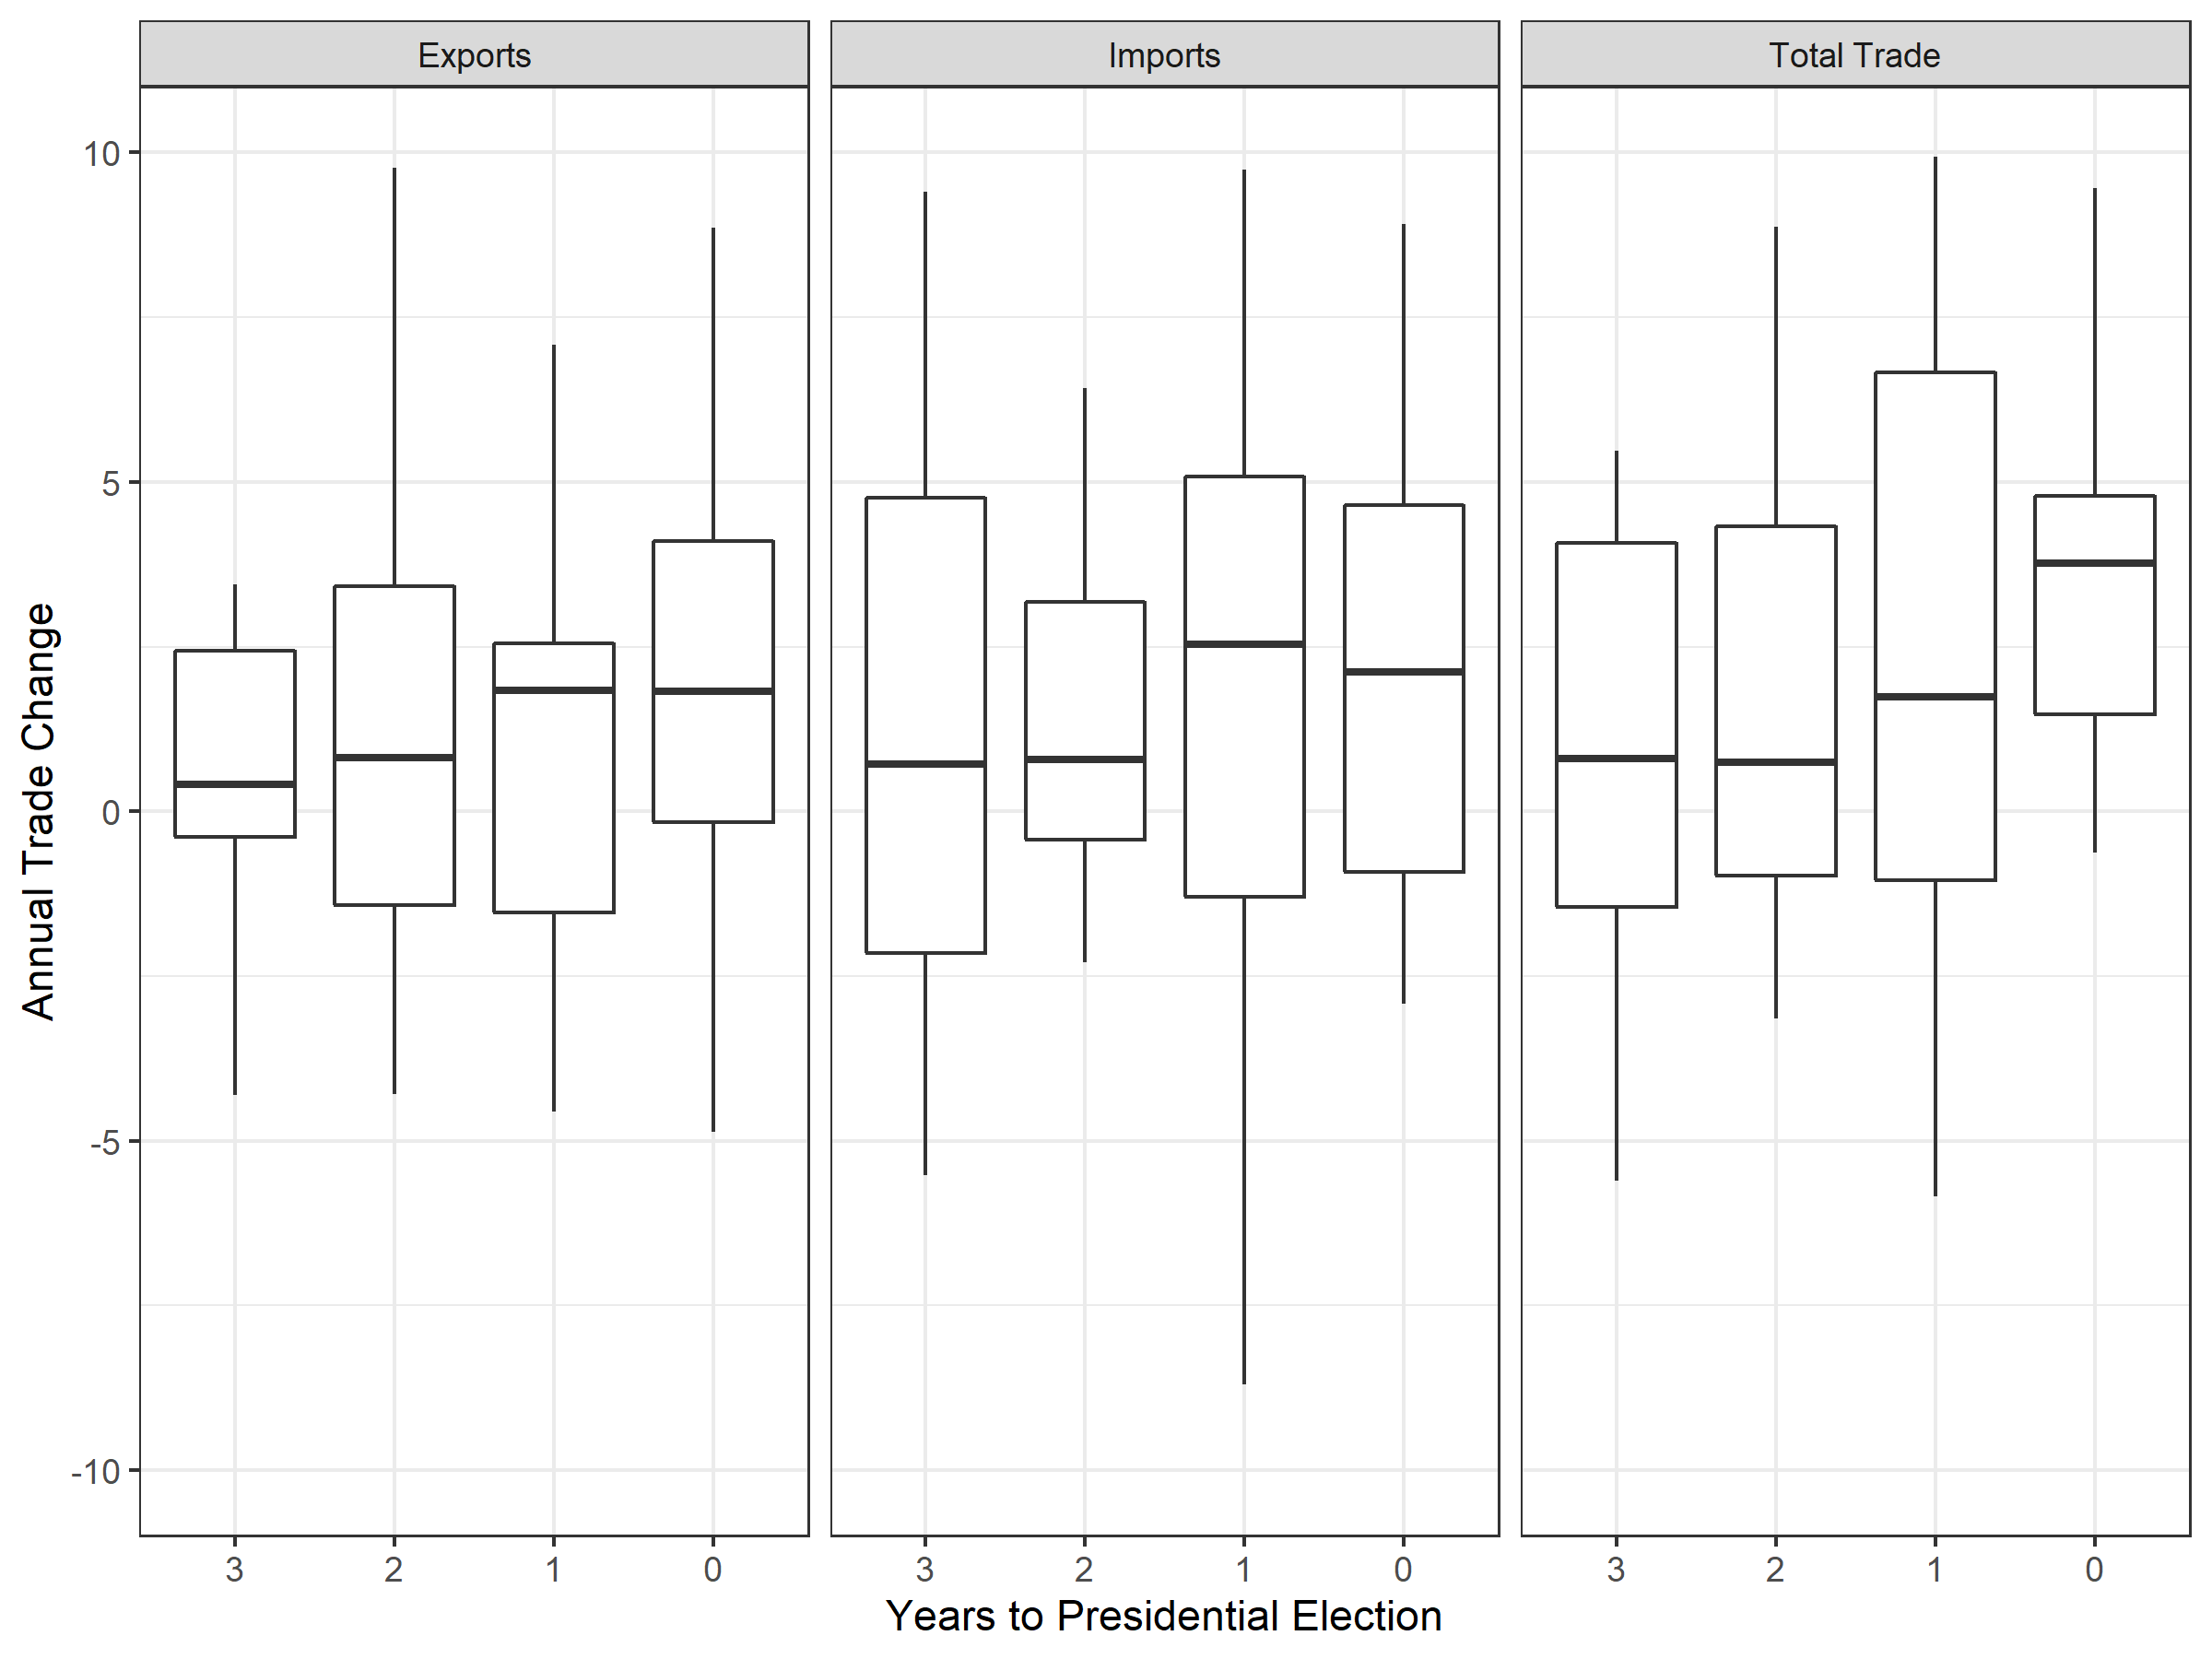
\includegraphics[width=0.95\textwidth]{../figures/us-trade-cycles.png}
\caption{Electoral cycles in U.S. trade between 1951 and 2019. Each box plot summarizes the distribution of changes in logged exports, imports, and overall trade as a presidential election approaches. The thick black line in each plot marks the median value.}
\label{fig:us-trade-cycles}
\end{figure}


While there is ample variation in export changes across, the median export change is highest in the year before or year of a presidential election.
Import changes also rise, though they vary more before an election. 
As a result of increasing exports and imports, total trade changes also increase, especially in presidential election years.


% targeted and flexible policies 
The economic roots of these electoral trade cycles are straightforward, the composition of electoral trade cycles requires further scrutiny.
Aggregate budgets often give leaders limited spending discretion, which leads to targeted spending shifts \citep[pg. 248]{Dubois2016}
Leaders also manipulate other policies such as trade disputes \citep{Conconietal2017}, labor agreements \citep{Ahlquist2010} and land reform \cite{Philips2020} to win support in key constituencies.


% Defense spending/contracts as flexible instrument
Although aggregate budgets are hard to manipulate, many observers claim that defense spending is more flexible instrument for budget cycles \citep{Tufte1978, Mintz1988}.
Executive leaders often have more discretion in how to allocate defense resources, and defense spending has economic ramifications.
\citet{WhittenWilliams2011} note that defense spending can serve social welfare goals. 
\citet{Becker2021} finds that unemployment in NATO members encourages leaders to shift spending from equipment to personnel.


% in US context, contracts
More recent work on the United States argues that defense budgets, which are set two years in advance, cannot drive political cycles.
As a result, attention shifted towards defense contracting, as leaders have more control over contract timing and disbursement \citep{Mayer1995, DerouenHeo2000}.
Disbursing contracts allows leaders to target key constituencies in response to unemployment and approval.


% increased production of arms- not tied to security needs
Defense contracting increases arms production by employing firms to produce defense goods. 
While these goods can equip the U.S. military, electoral cycles and defense planning may diverge.
Even the U.S. military may lack absorptive capacity to incorporate defense contracting outputs.
Put differently, increased supply from electoral cycles in defense contracting does not respond to increased military demand, requiring other buyers. 
Foreign markets provide alternative outlets for excess arms production from defense contracting cycles. 


% additional production and foreign markets
When defense production and planning diverge, foreign markets provide alternative takers for excess arms production from defense contracting cycles. 
Security partners are an especially pivotal outlet, because alliances promote security, economic and political cooperation.
Large states often transfer or sell arms to alliance proteges, and proteges have means and motivation to accommodate electoral cycles. 



\subsection{Alliances and Exports}


% basic asymm alliance framework
In asymmetric alliances between large and small states, the large state protects its smaller partner in exchange for foreign policy concessions \citep{Morrow1991}.
A credible promise of military support increases the large state's foreign policy influence. 
Small alliance members garner protection from external threats and sacrifice some foreign policy autonomy. 
Although many asymmetric alliance formalize hierarchical relationships, security and economic hierarchy are distinct \citep{Lake2009}. 


Military alliances and economic cooperation are inseparable.
Many alliances also include explicit or implicit promises of economic cooperation \citep{GowaMansfield2004, LongLeeds2006, Davis2008, Poast2012}.\footnote{Conflict and economic integration are linked in general (see for example, \citep{GartzkeLi2003, Chen2021}).}
Prior research indicates that alliances promote trade \citep{Gowa1995, GowaMansfield2004, Haim2016} or protect existing trade ties \citep{Fordham2010}.
Alliances also encourage foreign direct investment \citep{LiVashchilko2010} and monetary cooperation \citep{Li2003}.
A cooperative bargain of security and economic ties results. 


% potential markets: allies
% take new or used stuff to make room
U.S. allies are an obvious market for outputs from political cycles in defense contracting.
Close security cooperation and economic integration of defense industries create economic and security ties that encourage arms trade \citep{Bitzinger1994}. 
\citet{Thurneretal2019} find that while the relative importance of security and economic factors fluctuates, alliances consistently increase arms transfers.


% sending arms: political benefits for patron and proteges
Electoral cycles in arms transfers benefit U.S. and allied leaders.
Presidents gain additional flexibility to manipulate economic conditions and signal support for U.S. alliance proteges. 
\citet{McManusYarhi-Milo2017} argue that arms transfers are a costly but less visible signal of patron support.\footnote{\citet{Yarhi-Miloetal2016} argue that arms transfers sometimes substitute for alliances so patrons can provide security with less entrapment risk.}


% positive statecraft tie-in from Baldwin 
U.S. allies curry favor with their patron, bolster their military capabilities and deepen perceived commitment.
Accepting arms transfers is thus positive economic statecraft. 
Purchases and transfers are a common way that states bolster their political influence and power \citep[pg. 42-3]{Baldwin2020}.
In alliance politics, \citet[pg. 184-5]{IkenberryGrieco2003} note that states often use direct transfers to attract and sustain security commitments.  


Arms transfers fall under direct leader control in the protege, which gives flexibility to respond to defense contracting cycles in a patron.
Arms imports are also more flexible than tariffs or other trade policy, as the protege government has direct control over import decisions.
Just as political control of firms increases trade policy flexibility \citep{Davisetal2019}, governments are the customer for most arms sales or transfers. 


% Sales and transfers- who pays for what
Moreover, proteges do not always pay for U.S. arms transfers.
United States often subsidizes or gifts arms transfers through foreign military sales programs. 
While these still count as arms exports, they impose fewer immediate costs on recipients.
Regardless of the fiscal implications, allies are more likely to receive pure transfers or subsidies than other states.


% less export cycles to non-allies
The security externalities of arms transfers will reduce electoral cycles in arms exports to non-allies, however. 
U.S. leaders will be less willing to increase the capability of potential opponents, even if it facilitates electoral cycles.
Furthermore arms transfers outside of alliances may face greater opposition scrutiny near elections, so presidents may hold off on contentious arms transfers to forestall criticism.
Limited defense industry cooperation also constrains the set of potential exports to finished goods, while allies with defense industrial ties can send intermediate goods.


% Net implications: total trade increases and trade balances unchanged
I expect general trade increases and greater exports to allies through arms transfers around U.S. elections.
These flows impact overall trade volume and trade balances.
Greater imports and exports will increase total trade around elections. 
The relative impact on trade balances depends on whether imports or exports increase more. 
If U.S. proteges take more exports than non-allies, the U.S. trade balance with those states will improve relative to trade balances with non-allies however.


% Result- increased exports, tied to electoral cycles
The result of this process is increased trade as elections approach, especially exports from the United States to alliance proteges.
These electoral export cycles in alliances are the result of arms transfers. 
Arms transfers in turn are rooted in electoral cycles of defense contracting.




\subsection{Implications}



The argument generates several testable implications. 
Testing is most straightforward in states with a large economy, fixed electoral calendar and robust domestic defense industry. 
Therefore, this analysis focuses on the United States. 


The first hypothesis predicts general electoral cycles in trade, especially exports to allies. 
As presidential elections approach, I expect increasing exports from the United States to alliance proteges.


\begin{quote}
\textsc{Export Cycles Hypothesis: As time to a presidential election decreases, U.S. exports to junior allies will increase.}
\end{quote}



The second hypothesis predicts corresponding cycles in arms transfers.
If arms transfers and sales drive export cycles, electoral cycles in arms transfers should match trade cycles.
Proximity to presidential elections will increase arms transfers from the United States to allied states. 


\begin{quote}
\textsc{Arms Transfers Hypothesis: As time to a presidential election decreases, U.S. arms transfers to junior allies will increase.}
\end{quote}


The third prediction tests the expected relationship between defense contracts and arms exports. 
I expect electoral cycles in defense contacting, and a positive correlation between these cycles and U.S. arms transfers.


\begin{quote}
\textsc{Defense Contracts Hypothesis: As defense contracting increases around elections, U.S. arms transfers will increase.}
\end{quote}



In the following, I describe how I test each of these hypotheses. 
In the first analysis, I establish the role of allies in electoral export cycles. 
The second analysis shows increasing exports to allies track with the U.S. electoral cycles, and are of comparable magnitude to trade cycles.
Finally, I test the final link in the argument chain with an analysis of defense contracting and arms exports from YEAR TO YEAR.




\section{Electoral Cycles in U.S. Exports to Allies}

To test the first hypothesis, I analyze U.S. trade from 1950 to 2014. 
This analysis presents electoral trade cycles, then establishes that allies drive electoral export cycles.
The key independent variable is a dummy indicator of a defensive alliance between the United States and each state, drawn from the ATOP database \citep{Leedsetal2002}.
I then employ elections data from the National Elections across Democracy and Autocracy (NELDA) dataset \citep{HydeMarinov2012} to identify presidential election years and calculate years to the election.
The years to election variable ranges from zero in election years to three in the year immediately after an election.
Finally, I interact the defensive alliance dummy with the years to election variable.


For U.S. exports, my argument makes three predictions about the interaction between alliances and years to election. 
First a positive constituent term on the defensive alliance variable, which indicates that allies take more exports than non-allies in election years, when time to election is zero.
Second, I expect a negative constituent term on years to election as non-allied states respond to political business cycles in other ways.
Last, and most importantly, a negative interaction between alliances and time to the election, which suggests that exports to allies are more responsive to elections than exports to states without a defensive alliances with the United States.


The key outcome is annual changes in the natural log of exports, but I also model changes in total trade, imports, and the trade balance to assess the net impact of export changes.
I use changes because models in levels with a lagged dependent variable suggest non-stationarity in many panels. 
Because lagged trade flows have unit roots or near unit root coefficients, models in levels risk spurious inferences.
I draw on exports and imports data from the IMF's direction of trade statistics database.


In addition to the interaction of time to elections and a defensive alliance, I include a series of control variables that may be correlated with alliances and trade. 
Key trade variables include for changes in the GDP of both states, population-weighted distance, contiguity, common language and former colonial ties \citep{FouquinHugot2016}.
I also adjust for democracy \citep{Marquez2016}, the presence of a militarized interstate dispute \citep{Gibleretal2016}, and shared IGO membership \citep{Pevehouseetal2020}.\footnote{Some dyadic data from the \textit{peacesciencer} \textsf{R} package \citep{peacesciencer-package}.}


Some trade flow changes are unusual. 
This creates heavy-tailed residuals, so I employ a robust regression estimator; M-estimation with Tukey's biweight function \citep{RaineyBaissa2020}.
Robust regression places less weight on unusual observations, making it more efficient than OLS for this particular outcome.



\subsection{Results}


Raw trade data shows differences between allies and non-allies in electoral cycles in U.S. exports, imports and total trade. 
\autoref{fig:us-trade-cycles-all} presents the distribution of changes in logged exports, imports and overall trade in years with differing electoral proximity.
Box plots summarize the distribution of U.S. trade with all states in those years. 
The dark line in each box plot marks the median value. 



\begin{figure}
\centering
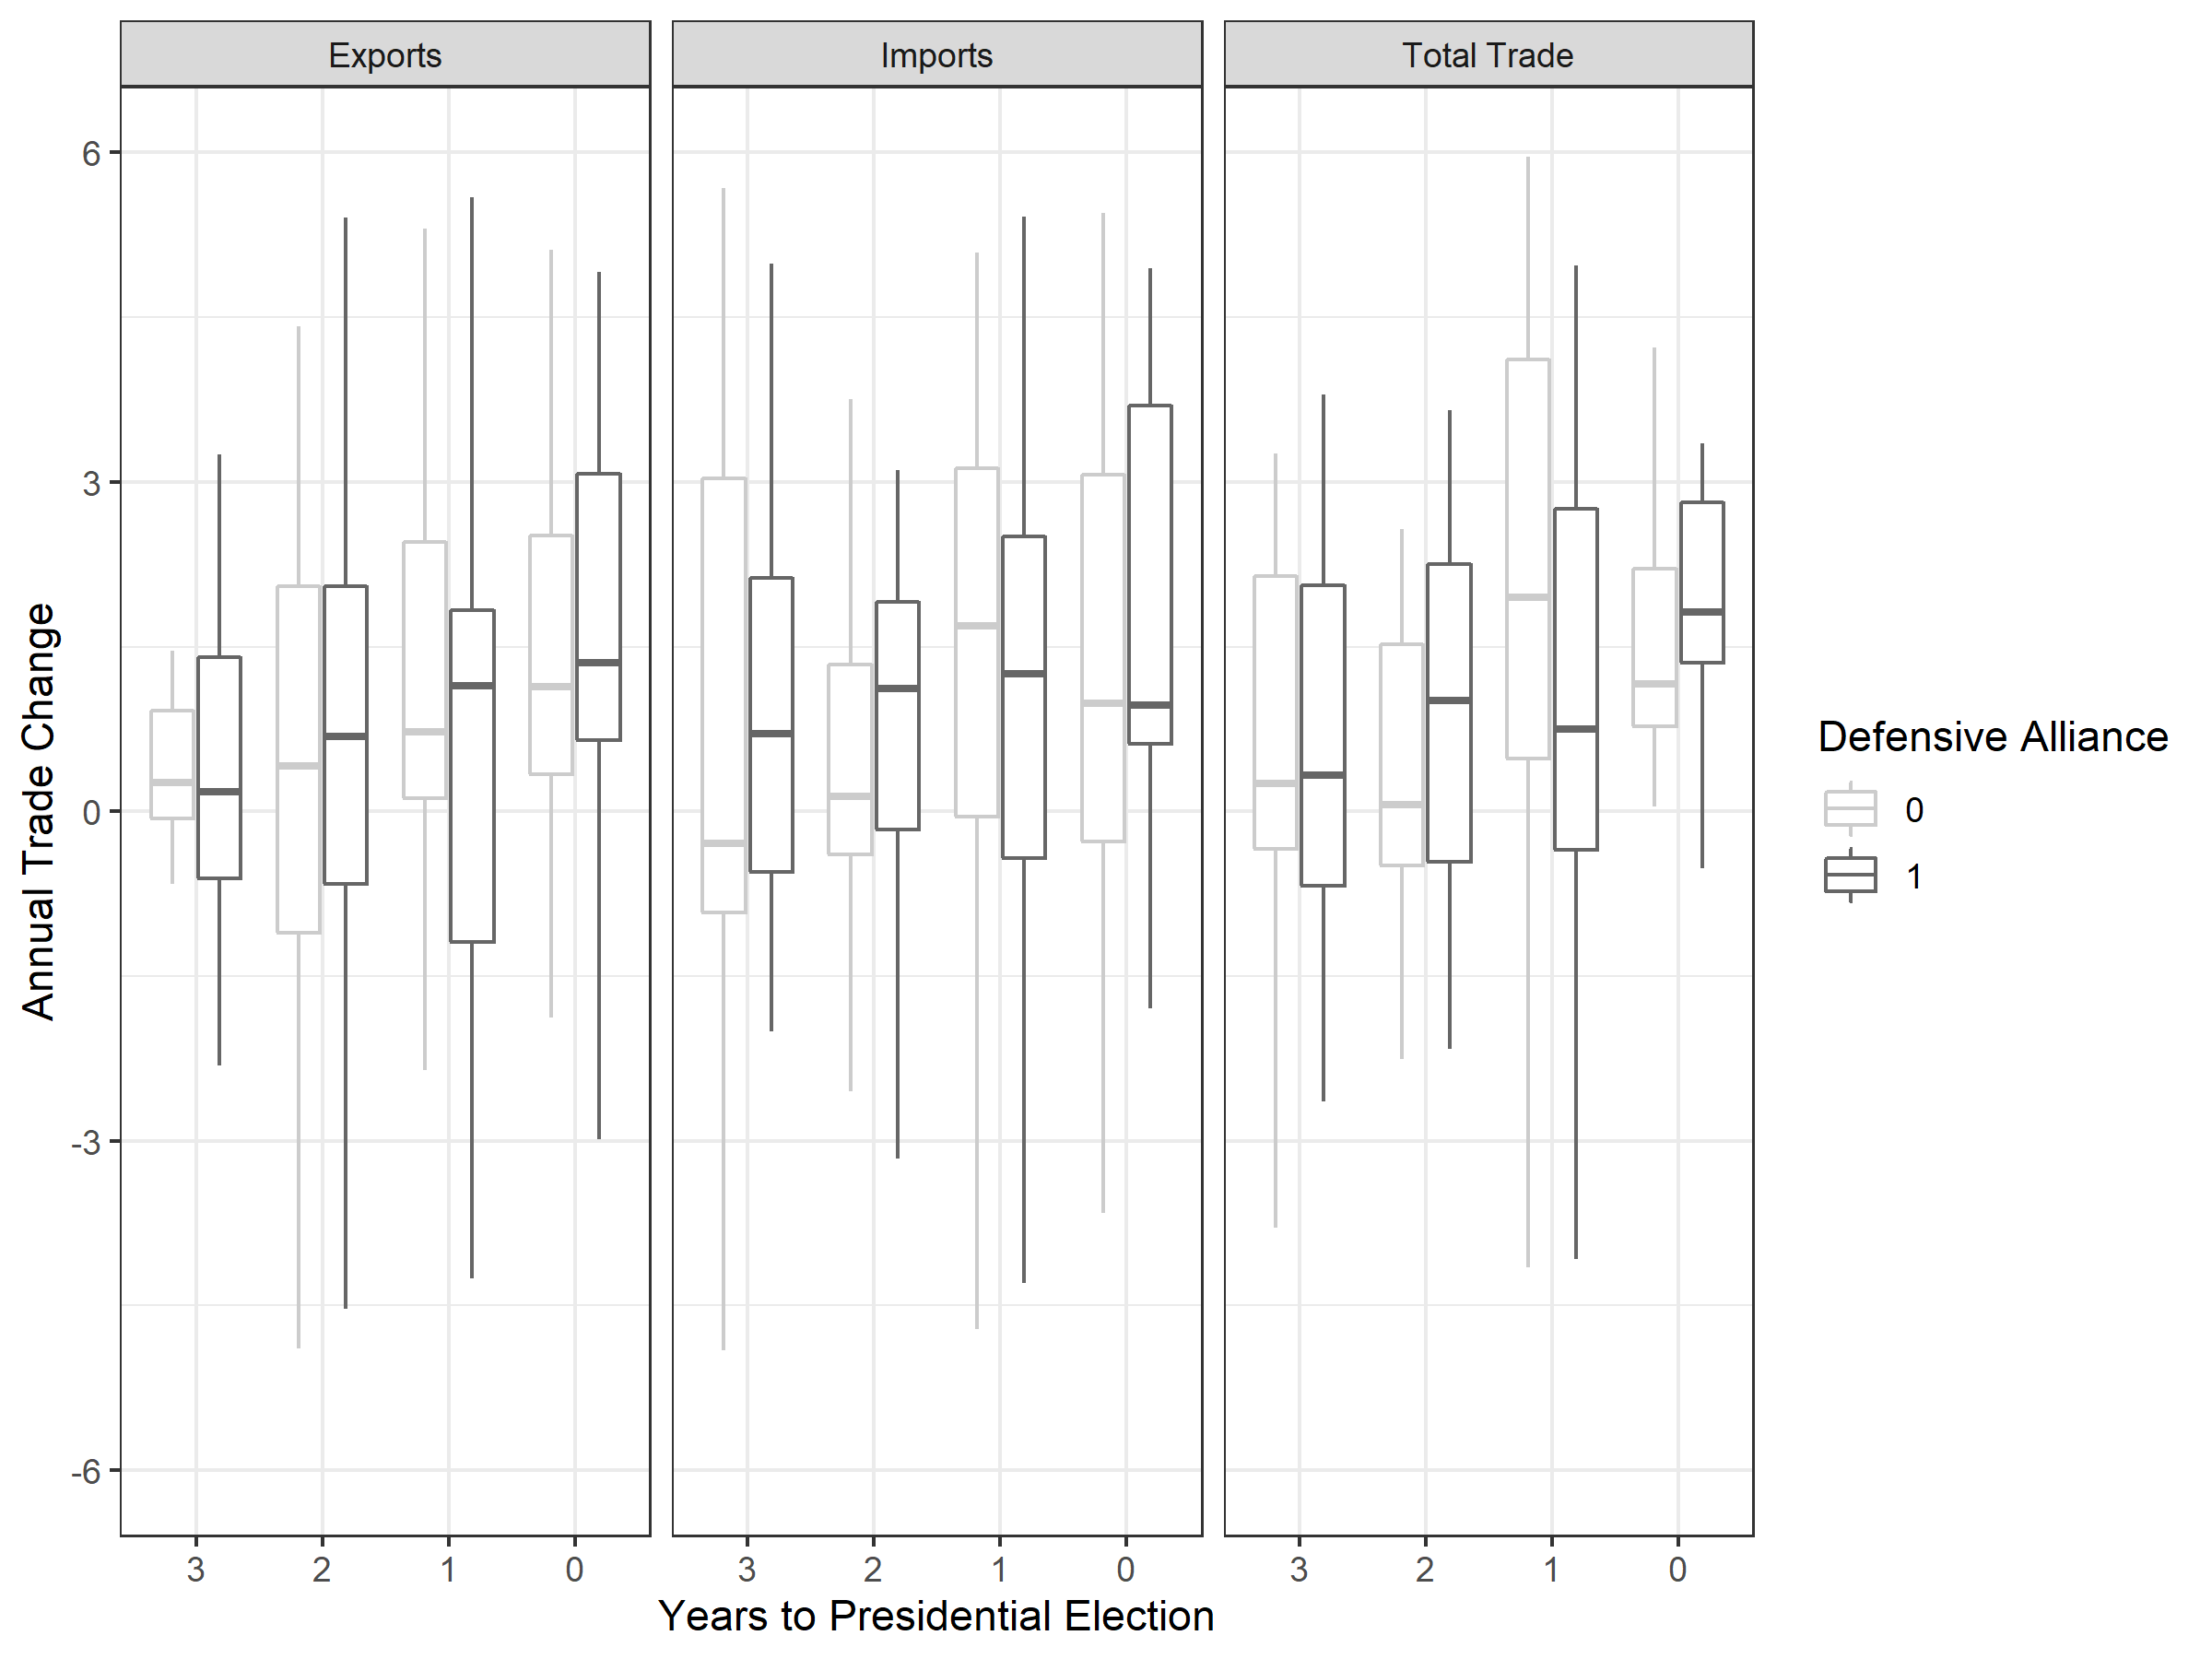
\includegraphics[width=0.95\textwidth]{../figures/us-trade-cycles-all.png}
\caption{Electoral cycles in U.S. trade between 1950 and 2014. Each box plot summarizes the distribution of changes in logged exports, imports, and overall trade as a presidential election approaches. Colors mark trade with allies and non-allies. The thick black line in each box plot marks the median value.}
\label{fig:us-trade-cycles-all}
\end{figure}


Median export changes are higher for allies than non-allies near presidential elections. 
Export changes for non-allies still rise, but less than exports to allies. 
Imports from non-allies and allies are equally responsive to election timing. 
As a result, total U.S. trade increases regardless of formal security ties.


\autoref{fig:us-trade-cycles} shows electoral cycles in U.S. trade, but it is possible that other factors confound this relationship.
\autoref{fig:us-trade-coefs} presents coefficient estimates from the robust regression models. along with 95\% confidence intervals in parentheses. 
These estimates suggest that allies drive U.S. export cycles, but all states respond to elections with increased exports to the United States. 


\begin{figure}
\centering
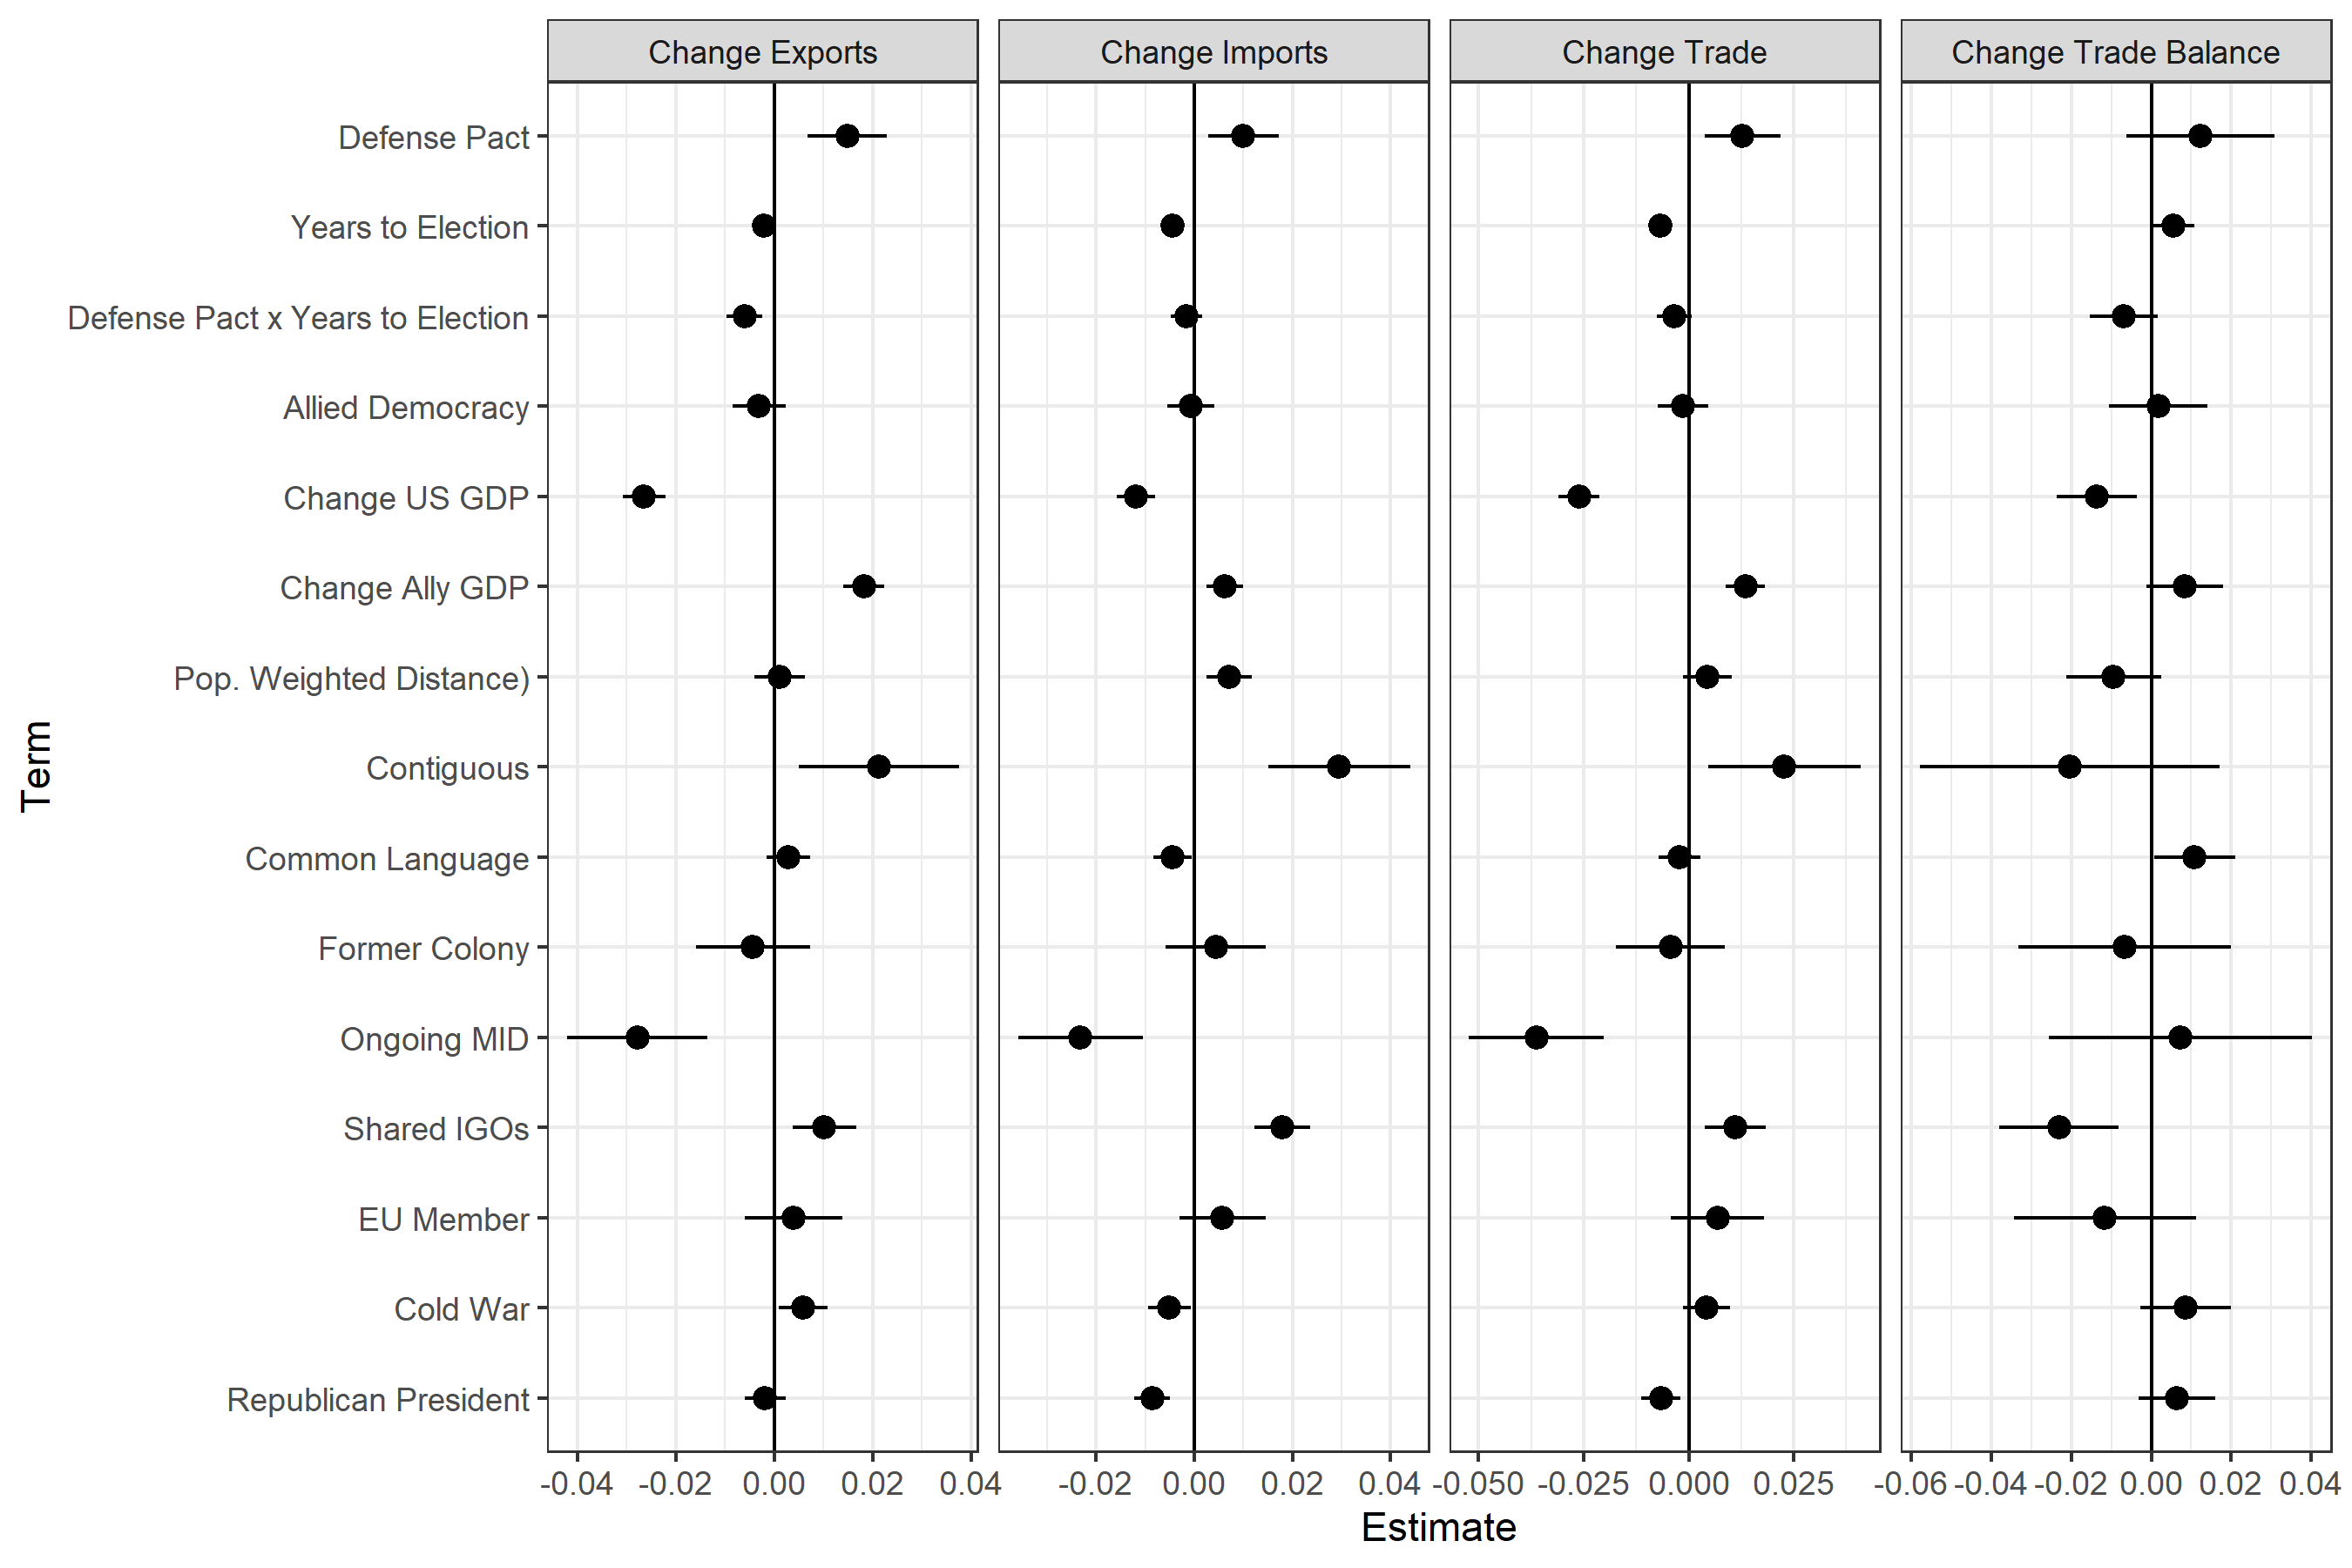
\includegraphics[width=0.95\textwidth]{../figures/us-trade-coefs.png}
\caption{Robust regression coefficients from models of U.S. trade, 1950 to 2014. Points mark coefficient estimates and error bars encapsulate 95\% confidence intervals. All continuous predictors rescaled by two standard deviations.}
\label{fig:us-trade-coefs}
\end{figure}


As expected, the interaction between the defensive alliance dummy and years to election is negative, which implies that allies receive more U.S. exports as presidential elections approach.
Allies receive more U.S. exports in general, and respond especially strongly to elections when doing so.


The interaction term for imports suggests no clear difference in U.S. imports around elections between allies and non-allied states. 
Moreover, the time to election constituent term is negative for all outcomes, except the trade balance. 
Trade changes approximate the track of exports. 
Simultaneous increases in imports and exports have a more uncertain impact on trade balances.
 


% predicted
The sign and confidence intervals of the interaction terms are inadequate evidence of a conditional relationship \citep{BramborClarkGolder2006}, so I plot predicted changes in trade flows in \autoref{fig:us-elec-pred}.
This figure presents predicted changes in trade across time to election for states with and without a U.S. defense pact. 
Given non-linear relationships from logged trade flows and a robust estimator, these predictions are more straightforward to interpret than marginal effects.\footnote{I present marginal effects in the appendix.} 


\begin{figure}[htpb]
	\centering
		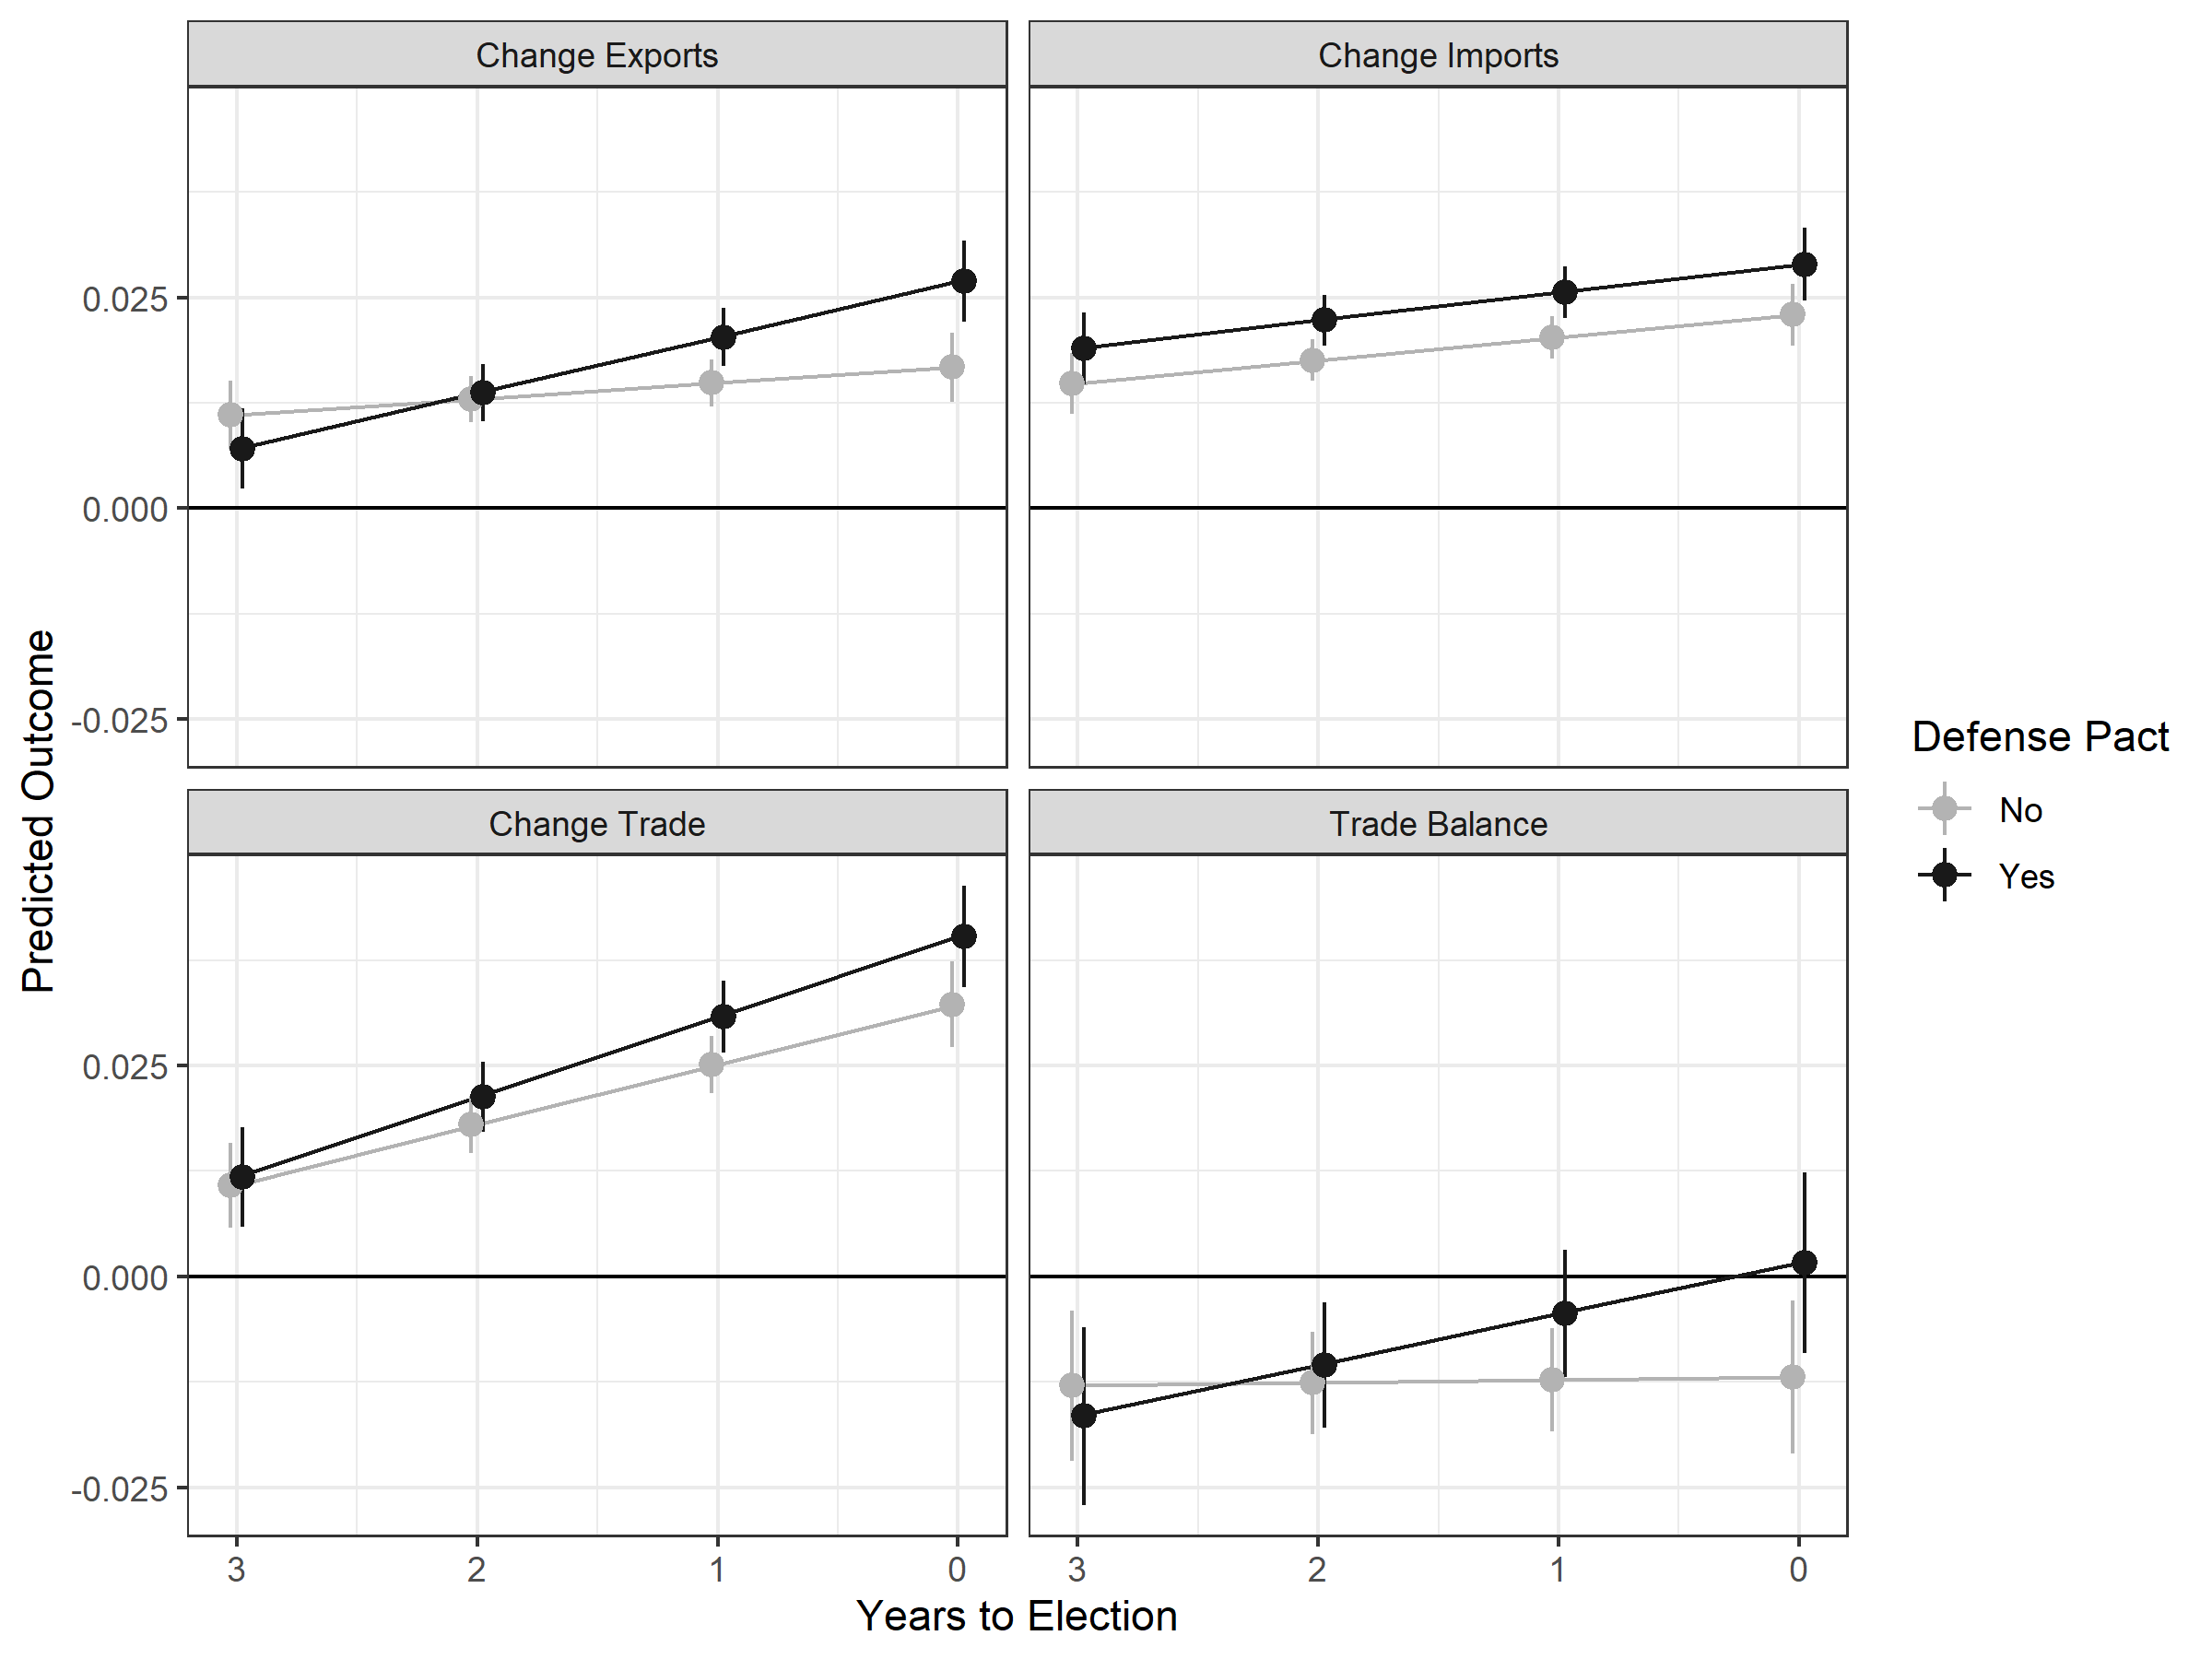
\includegraphics[width=0.95\textwidth]{../figures/us-elec-pred.png}
	\caption{Predicted changes in trade between the the United States and other states. Points mark the predictions and error bars summarize the 95\% confidence interval.}
	\label{fig:us-elec-pred}
\end{figure}


The predicted changes in exports, imports, total trade and the trade balance are consistent with inferences from the coefficient estimates. 
While U.S. exports to non-allies rise somewhat with election proximity, exports to allied states rise far more. 
Allied and non-allied export changes are comparable until the year before and year of U.S. presidential elections, and after that, allied exports increase by far more. 


% time to election
U.S. imports increase as presidential elections approach, and there is little difference in the trend between allies and other states. 
This is the result of political budget cycles boosting domestic consumption, which do not target specific goods.
Imports from allies are consistently greater than imports from non-allies, however, which is consistent with prior work on alliances and trade promotion \citep{GowaMansfield2004}. 


Differences in exports produce distinct electoral trade cycles between states with a U.S. defense treaty and those without. 
Non-allies increase imports and exports in similar ways as elections approach. 
As a result, their total trade changes increase with election proximity, but less so than allies. 


Trade balances, a common concern among some policymakers, show less evidence of electoral cycles. 
U.S. trade deficits with allies narrow somewhat around elections, but expand with non-allies, as imports rise more than exports. 
Uncertainty in these estimates makes distinguishing the estimates between and within the two groups difficult.


% improved trade balance
These results are consistent with the export cycles hypothesis. 
Exports to allies increase more near elections than exports to non-allies.
In the next section, I show that these differences in exports are the result of arms transfers, and transfers follow from increased defense contracting.



\section{Arms Transfers and Presidential Elections}


I model arms transfers using data from the SIPRI Arms Transfer Database \citep{SIPRI2021}.
The outcome in this analysis is annual logged arms transfers, based on SIPRI's trend indicator value methodology for the major conventional weapons.
I model arms transfer levels because these shifts are less autocorrelated than overall exports.
I cannot use the same estimation strategy, however, because 60\% of the observations have zero observed arms transfers, and thus a change of zero.
Such zero-inflation makes standard regression techniques impractical.
To overcome this issue, I use a two-stage model. 


In the first stage, I model a binary indicator of non-zero arms transfers with a logistic regression. 
The logistic regression predicts U.S. arms transfer presence with the defensive alliance dummy, dummy indicators of the Cold War, EU membership and Republican presidencies, recipient democracy, shared IGO membership and MID participation. 
I also include indicators of U.S. and recipient GDP, population-weighted distance, along with binary measures of common language, contiguity and colonial history. 
Finally, I account for duration dependence with cubic time polynomials \citep{CarterSignorino2010}.


The second stage model is a robust regression --M-estimation with Tukey's biweight function-- of all non-zero changes in arms that adds the predicted probability of non-zero arms transfers and a lagged arms transfer indicator to the predictors from the model of changes in exports.
I interact defense pacts and time to election to capture differences in electoral cycles between U.S. allies and non-allies. 
Other controls match the exports model, encapsulating economic, cultural, and distance in ties between the United States and other states. 
As a result, this model approximates a hurdle from zero to positive arms transfers.


\subsection{Results}


These results proceed in two parts.
First, I present the coefficient estimates from the logistic regression of arms transfer presence and robust regression of elections, alliances and arms transfer changes in \autoref{fig:us-trade-cycles}.
I then summarize the interaction of alliances and presidential election proximity in \autoref{fig:us-arms-plots}.


At the arms transfer hurdle stage, defense pacts increase the likelihood of arms transfers, as does contiguity, shared IGO membership, and former colonial ties.
Increasing allied GDP increases the likelihood of arms transfers.
More distant states are also more likely to receive arms transfers, as the United States sells many arms outside the Western Hemisphere. 
After accounting for alliances, increasing democracy and U.S. GDP make arms transfers less likely, as did the Cold War. 
The negative Cold War coefficient reflects greater dispersion in U.S. arms transfers across multiple states after the USSR collapsed.


\begin{table}
\centering
\resizebox{\textwidth}{!}{
\begin{tabular}[t]{lcc}
\toprule
  & Non-Zero Arms Transfer: Logit & Arms Transfers: Robust Reg\\
\midrule
Defense Pact & 1.61 & 0.34\\
 & (1.43, 1.79) & (0.13, 0.56)\\
Years to Election &  & 0.04\\
 &  & (-0.02, 0.10)\\
Defense Pact x Years to Election &  & -0.08\\
 &  & (-0.16, -0.01)\\
Partner Democracy & -0.34 & -0.01\\
 & (-0.51, -0.18) & (-0.12, 0.11)\\
US GDP & -0.50 & -0.19\\
 & (-0.76, -0.25) & (-0.37, -0.01)\\
Partner GDP & 0.24 & 0.09\\
 & (0.06, 0.42) & (0.01, 0.18)\\
Pop. Weighted Distance) & 1.39 & 0.49\\
 & (1.23, 1.56) & (0.33, 0.65)\\
Contiguous & 1.12 & 0.59\\
 & (0.53, 1.78) & (0.32, 0.86)\\
Common Language & -0.04 & -0.22\\
 & (-0.17, 0.09) & (-0.31, -0.12)\\
Former Colony & 1.00 & 0.22\\
 & (0.50, 1.54) & (0.04, 0.40)\\
Ongoing MID & -0.81 & -0.20\\
 & (-1.23, -0.40) & (-0.55, 0.15)\\
Shared IGOs & 2.63 & 0.54\\
 & (2.40, 2.87) & (0.25, 0.83)\\
EU Member & -0.20 & -0.30\\
 & (-0.52, 0.14) & (-0.48, -0.12)\\
Cold War & -0.80 & -0.18\\
 & (-1.04, -0.56) & (-0.37, 0.02)\\
Republican President & -0.10 & -0.03\\
 & (-0.23, 0.02) & (-0.12, 0.06)\\
Lag Ln(Arms Transfers) &  & 0.61\\
 &  & (0.58, 0.63)\\
Pred. Prob. of Arms Transfer &  & -0.65\\
 &  & (-1.21, -0.09)\\
\midrule
Num.Obs. & 7879 & 3268\\
\bottomrule
\end{tabular}
}
\caption{Coefficient estimates from a logistic regression of non-zero U.S. arms transfers and robust regression of changes in arms transfers. All continuous predictors rescaled by two standard deviations. Intercepts included but omitted from the table. The logit model estimates also omit the cubic time polynomials.}
\label{tab:arms-ch-hurdle}
\end{table}


In the robust regression of arms transfer changes, states with a U.S. defense pact receive greater arms transfer changes in presidential election years. 
As with overall exports, the difference between allies and non-allies decreases as time to an election increases.
The key difference with the overall exports finding is that arms transfers to non-allies fall as presidential elections approach. 
This suggests that increasing exports from non-allies to the United States around elections in \autoref{fig:us-elec-pred} concentrate in other goods. 


Alliances and elections are not the only meaningful predictors of arms transfers.
The level of arms transfers is less sensitive to partner democracy, but it increases with allied GDP and decreases with U.S. GDP. 
Contiguous, more distant and former colony states also receive more transfers, as do states that share more IGO membership with the United States.
The predicted probability of arms transfer coefficient implies that states that were more likely to receive arms are less likely to see large increases in arms. 
Large increases in U.S. GDP reduce arms exports changes. 
The Cold War coefficient is largely negative, perhaps as the scale of arms transfers was more limited in that period. 
Last, there is some temporal autocorrelation in arms transfers, as the lagged dependent variable  


Again, the coefficient estimates in \autoref{tab:arms-ch-hurdle} are imperfect indicators of how alliances and electoral proximity interact.
\autoref{fig:us-arms-plots} therefore plots the predicted outcome and marginal effect of defense pacts based on the robust regression estimates.
These predicted changes in arms transfers and estimated marginal effect of defensive alliances match the regression coefficients.


\begin{figure}[htpb]
	\centering
		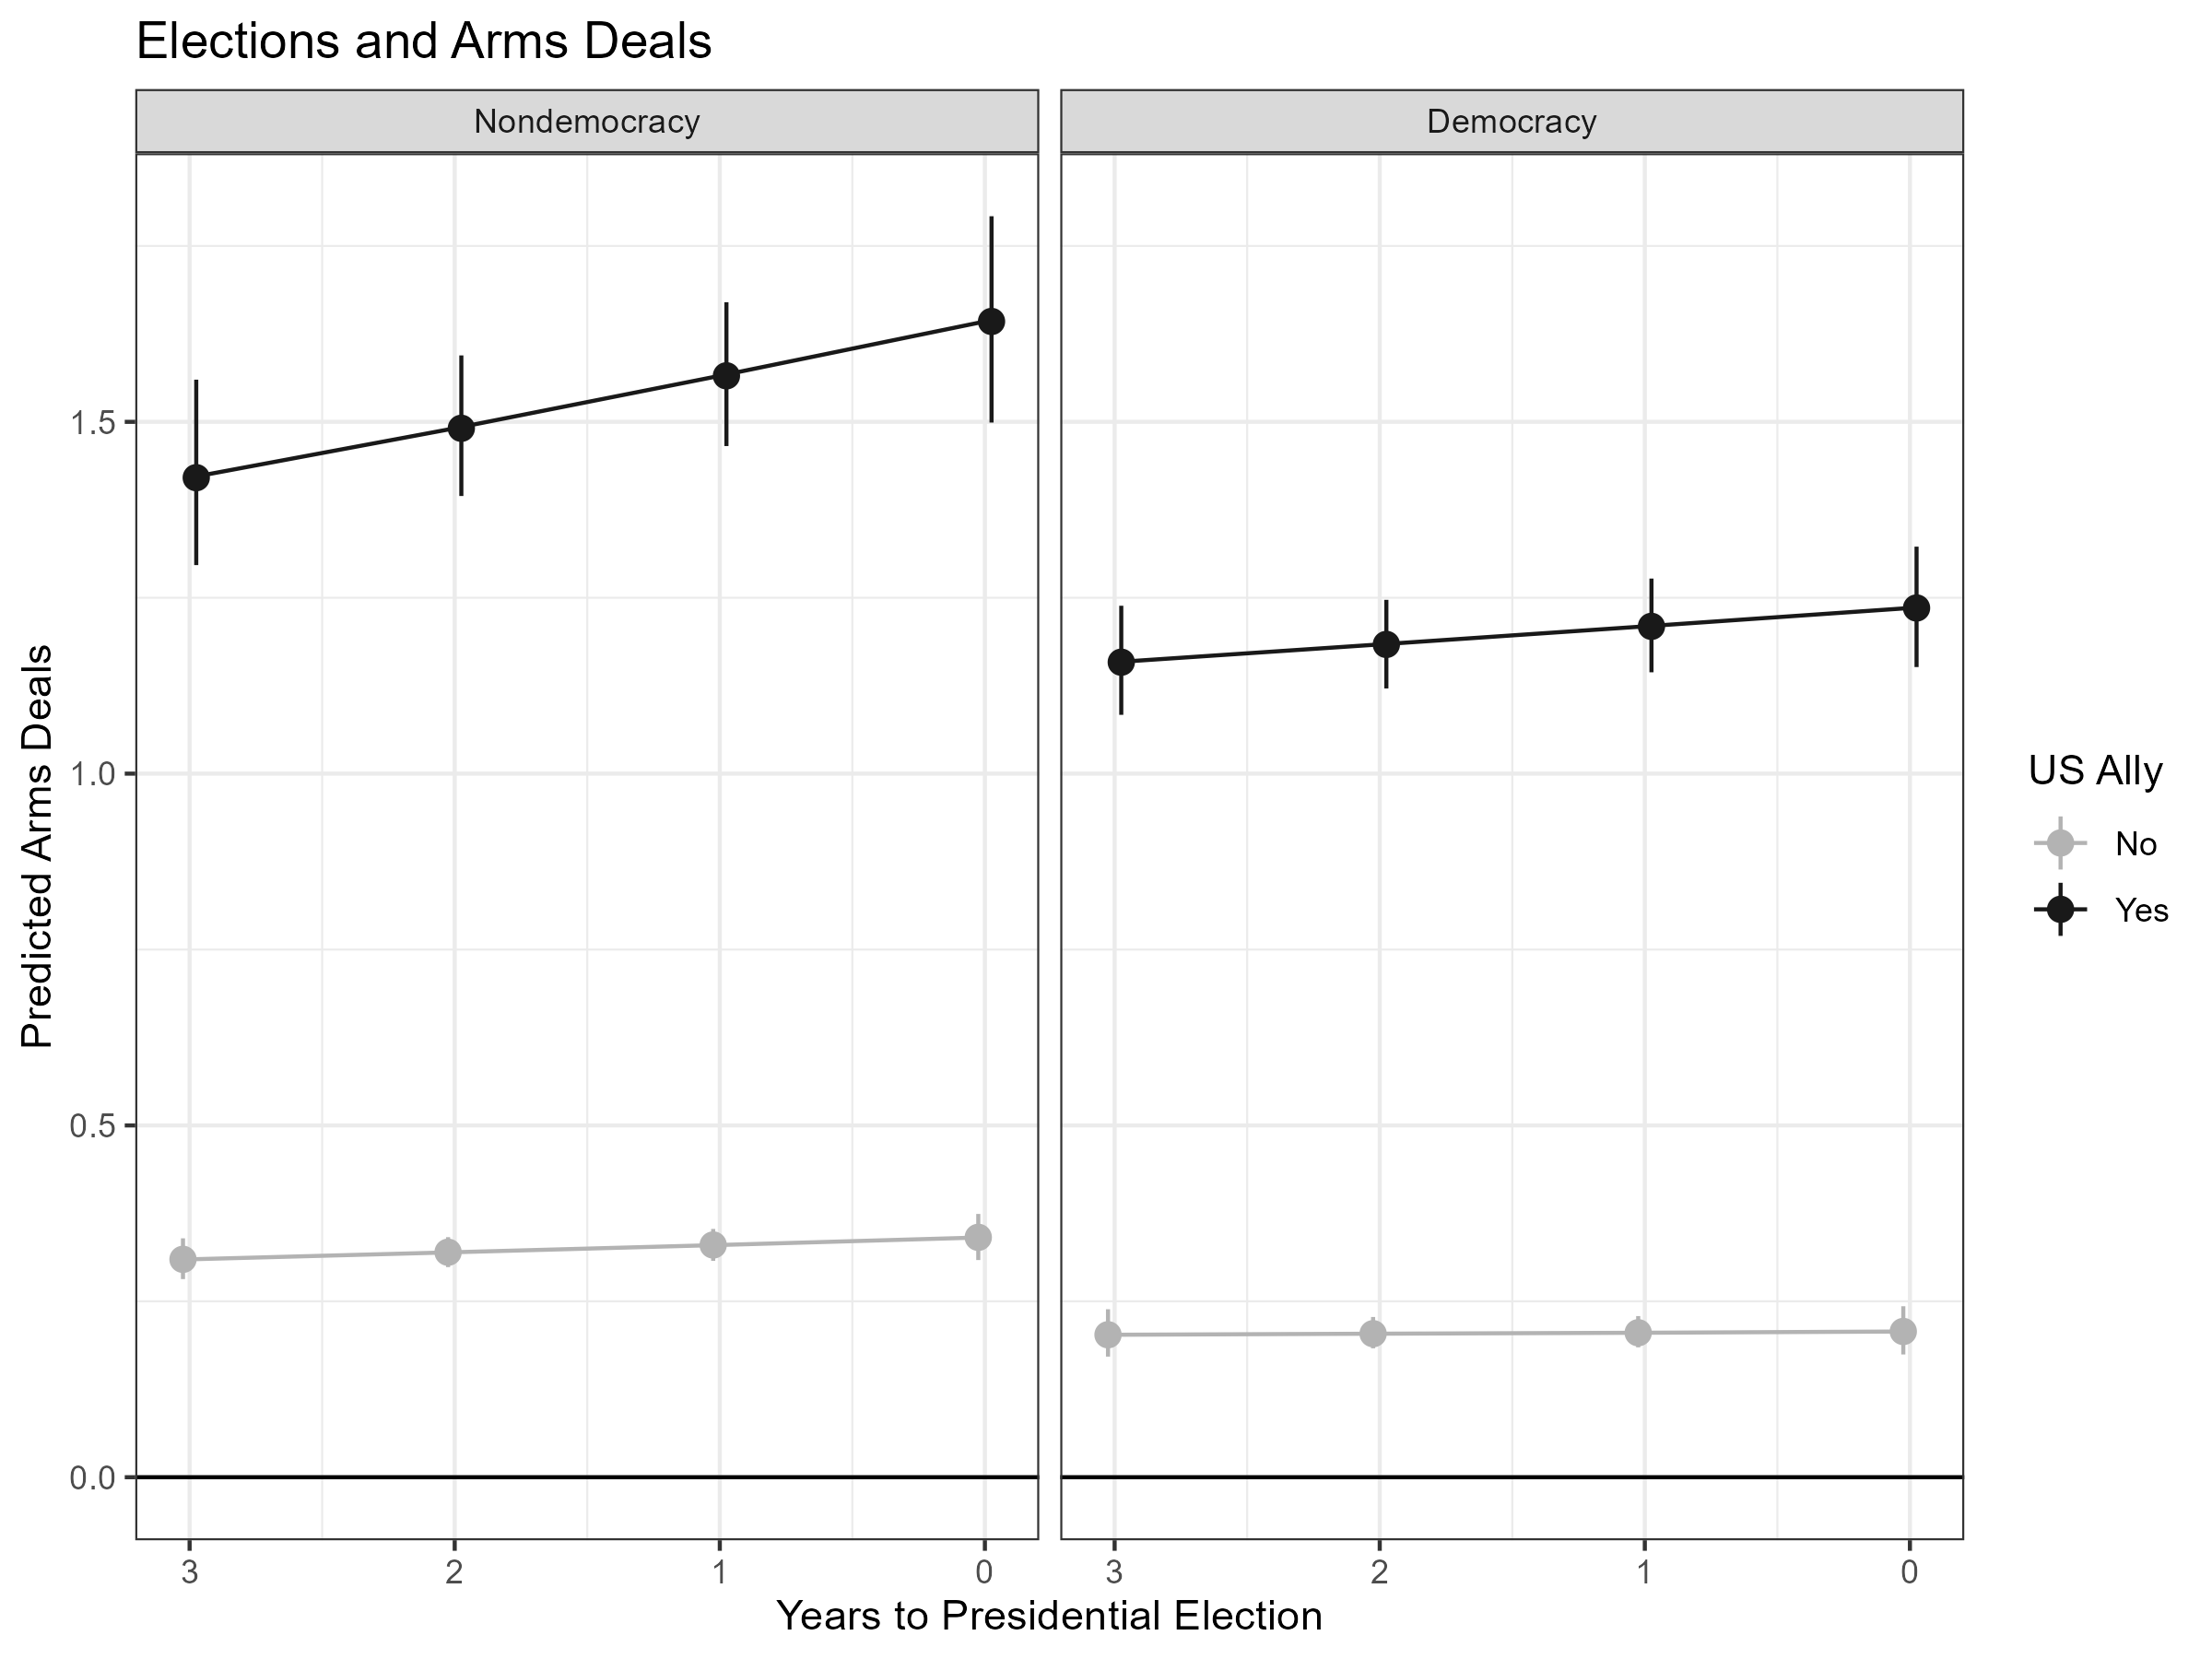
\includegraphics[width=0.95\textwidth]{../figures/us-arms-plots.png}
	\caption{Predicted out and the marginal impact of defensive alliances on changes in the log of arms transfers between the United States and other states 1950 to 2014. Points mark the estimates and error bars summarize the 95\% confidence interval.}
	\label{fig:us-arms-plots}
\end{figure}


First, predicted arms transfers to U.S. allies increase as presidential elections approach.
For a U.S. ally, predicted arms transfers rise by .14 in expectation. 
This is roughly equal to the marginal effect of an alliance on overall exports reflected in \autoref{fig:us-elec-pred}.
At the same time, arms transfers to non-allies fall as elections approach. 


As a result, while arms transfers to allies and non-allies are similar in the year after a presidential election, there is an expected gap of .34 between allies and non-allies in election years.
This is reflected in the marginal impact of a defense pact on arms transfers, which rises as presidential elections draw closer.


These divergent electoral cycles in arms transfers reflect divergent political relations.
Allies have more to gain from accommodating electoral cycles in arms transfers, and can fit additional U.S. arms into their forces that already use more U.S. kit.
Arms transfers cement cooperative relationships and bolster allied security through additional capability.
Leaders may also face more scrutiny over arms transfers outside alliances as elections approach. 




\section{Discussion and Conclusion}


All three results are consistent with temporary and targeted economic concessions to support committed leaders of large alliance members around elections. 
In the appendix, I check these findings.
First, I present alternative model specifications that find similar conditional relationships.
%check for non-linear relationships and adequate support in the interactions \citep{Hainmuelleretal2019}. 
%I also present inferences from Bayesian models that adjust for dyadic clustering through varying intercepts.


Demonstrating alliance commitment aids credible security commitments and provides contingent economic leverage. 
Alliance patrons have limited economic leverage, save when allies make temporary economic concessions to help them remain in office. 
Outside of election years, reassuring allies decreases democratic major power exports.
But when leaders offer more support, exports to allies hold up in election years and may concentrate in key constituencies.


Both perspectives on relative economic leverage in asymmetric alliances thus have some validity. 
Demonstrating security commitment often reduces exports and has no impact on allied tariffs. 
At the same time, leaders can leverage security commitments to garner allied support during elections. 


Alliances can therefore help leaders manipulate economic conditions to improve their electoral prospects. 
This finding adds an international mechanism to the political budget cycle literature.
Leaders can use international cooperation in non-economic issues to encourage other states to implement favorable economic policies. 


The argument and results reflect a general phenomenon that is more pronounced in alliances due to close economic and security relations. 
States regularly manipulate international economic ties to bolster or undermine leaders depending on their perceived stance on other issues. 
To give one example, \citet{ChyzhUrbatsch2021} show that Chinese soy tariffs reduced support for Republicans in the 2018 midterm elections. 
Allies have both motive and means to undertake similar actions. 
The security benefits of a cooperative leader motivate economic changes, and allies have many economic ties to leverage when they want to help a friendly leader. 
Future research should examine this phenomenon outside of military alliances.


These results also have implications for democratic alliance credibility and maintenance. 
A stable alliance bargain can develop if leaders anticipate the potential electoral benefits of economic ties with allies.
When leaders expect that demonstrating commitment will have electoral rewards, they will be more likely to invest in alliances. 
This also makes tolerating reduced trade leverage outside of elections worthwhile for patron state leaders.


In addition to assessing how states manipulate economic ties to support friendly leaders, future research could proceed in several directions. 
This paper presents some macro correlations, but could benefit from micro foundations. 
Are individuals more willing to make temporary economic changes that disadvantage domestic firms to support a friendly leader? 
When and how economic ties encourage alliance investments also merits further investigation.
Whether these results generalize to autocratic alliances is another worthwhile inquiry. 


In conclusion, large alliances leaders have limited and conditional economic leverage that depends on political leaders' commitment reputation and leadership competition. 
When a leader makes alliance investments, their exports to allied states increase during election years, and may concentrate in swing states. 
Otherwise, commitment reduces exports, and has no impact on structural policies like tariffs regardless of electoral pressure. 
Security preponderance thus provides less economic leverage than many observers expect, but still grants influence at critical junctures.


\newpage
\singlespace
 
\bibliography{../../MasterBibliography} 


\end{document}